\documentclass{article}
\usepackage{amsmath,graphicx}
\usepackage{cite}
\usepackage{amsthm,amssymb,amsfonts}
\usepackage{textcomp}
\usepackage{bm,enumerate}
\usepackage{algorithm}    
\usepackage{algorithmic}
\usepackage{booktabs}

\begin{document}

\title{Machine Learning, Spring 2018\\Homework 4}
\date{Due on 23:59 May 1, 2018\\Send to $cs282\_01@163.com$ \\with subject "Chinese name+student number+HW4"}
\maketitle




\section{Hoeffding Inequality}

\begin{enumerate}[(1)]
% \item Using binomial distribution, find the probability that a sample of 10 marbles will have $v \leq 0.1$ given that $\mu = 0.9$. (15 points)
\item ${\displaystyle \operatorname {P} ({v\leq 0.1)={\binom {10}{0}}\mu ^{0}(1-\mu)^{10}} + {\binom {10}{1}}\mu ^{1}(1-\mu)^{9}} = 9.1\times 10^{-9}$
% \item Using Hoeffding Inequality to bound the probability that a sample of 10 marbles will have $v \leq 0.1$ given that $\mu = 0.9$. (15 points)
\item $\because {\displaystyle \operatorname {P} [|v-\mu |>\varepsilon ]\leq 2\exp \left(-2\varepsilon ^{2}N\right)}$\\
Set $\varepsilon = 0.8$, then we get the bound is \\
$2\exp \left(-2\varepsilon ^{2}N\right) = 2\exp \left(-2\times 0.8 ^{2}\times 10\right) = 5.5\times 10^{-6}$
\end{enumerate}



\section{Bias-variance decomposition}
% \label{problem1}
% For a random variable $z$, let $\bar z$ denote its mean. Suppose our observation is generated by the true function $f$ as
% $$
% y = f(x) +\epsilon,
% $$
% where $\epsilon$ is normally distributed with zero mean and standard deviation $\sigma$. Training data set is $\mathcal{D}=\{x^{(i)},y^{(i)}\}_{i=1}^m$, from which you learned your hypothesis function $h_{\mathcal{D}}$. The bias-variance tradeoff is an important aspect of data science projects based on machine learning. 

% Now for a new data point $x^*$ out of $\mathcal{D}$, we want to investigate the expected error between the predicted value and the observation $y^*$, i.e.,
% $$
% \mathbb{E}_{\mathcal{D},\epsilon}[(y^*-h(x^*))^2].
% $$
% This error can be decomposed into three parts namely: \textbf{variance}, $\textbf{bias}^2$, and \textbf{noise}, where the expectation is taken over all possible training set $\mathcal{D}$. Here
% $$\begin{aligned} 
% \textbf{variance} &=\ \mathbb{E}_{\mathcal{D}}[(h(x^*)-\overline{h(x^*)})^2]\\
% \textbf{bias}^2 &=\ [\overline{h(x^*)}-f(x^*)]\\
% \textbf{noise} &=\ \sigma^2
% \end{aligned}
% $$
% with $\overline{h(x^*)}=\mathbb{E}_{\mathcal{D}}h(x^*)$.
% %$$
% %\textbf{variance} = \mathbb{E}_{\mathcal{D}}[(h(x^*)-\overline{h(x^*)})^2]
% %$$
% %$$
% %\textbf{bias}^2 = [\overline{h(x^*)}-f(x^*)]
% %$$
% %$$
% %\textbf{noise} =\sigma^2
% %$$
% %with $\overline{h(x^*)}=\mathbb{E}_{\mathcal{D}}h(x^*)$.
 
% The error \textbf{bias} is the amount by which the expected model prediction differs from the true value or target; while \textbf{variance} measures how inconsistent are the predictions from 1one another, over different training sets, not whether they are accurate or not. \textbf{Models that exhibit small variance and high bias underfit the truth target. Models that exhibit high variance and low bias overfit the truth target}.

% The data scientist’s goal is to simultaneously reduce bias and variance as much as possible in order to obtain as accurate model as is feasible. However, there is a tradeoff to be made when selecting models of different flexibility or complexity and in selecting appropriate training sets to minimize these sources of error.

% \textbf{Question}: 

% Show that
% $$
% \mathbb{E}_{\mathcal{D},\epsilon}[(y^*-h(x^*))^2] = \textbf{variance}+\textbf{bias}^2+\sigma^2.
% $$

% Hints: first you may want to prove a lemma that for any random variable, it holds true that
% $$
% \mathbb{E}[(z-\bar z)^2] = \mathbb{E}[z^2]-\bar{z}^2,
% $$
% so that
% $$
% \mathbb{E}[z^2]=\mathbb{E}[(z-\bar z)^2+\bar{z}^2].
% $$
% It follows that $(y^*-h(x^*))^2 = (y^*)^2 - 2h(x^*)y^*+h(x^*)^2$. Note that $y^*$ and $h(x^*)$ are independent variables. The result follows from using the lemma twice. Also note $\mathbb{E}_{\epsilon}[(y^*-f(x^*))^2]=\sigma^2$.  (20 points)
 \begin{enumerate}[(1)]
\item \textbf{Lemma:} $Var(z) = \mathbb{E}[(z-\bar z)^2] = \mathbb{E}[z^2]-\bar{z}^2$
\begin{proof}
$$Var(z) = \mathbb{E}[(z-\bar z)^2] = \mathbb{E}[z^2+\bar z^2 - 2z\bar z] = \mathbb{E}[z^2] + \bar z^2 - 2\bar z^2 = \mathbb{E}[z^2]-\bar{z}^2$$
\end{proof}
Then, show that $\textbf{variance}+\textbf{bias}^2+\sigma^2 = \mathbb{E}_{\mathcal{D},\epsilon}[(y^*-h(x^*))^2]$
\begin{proof}
	$$\overline{y^*} = \overline{f(x^*) + \epsilon} = \overline{f(x^*)} + 0 = f(x^*)\Rightarrow \overline{y^*} = f(x^*)$$
	\begin{equation}
		\begin{aligned}
		\textbf{variance}+\textbf{bias}^2+\sigma^2 &= \mathbb{E}_{\mathcal{D}}[(h(x^*)-\overline{h(x^*)})^2] + [\overline{h(x^*)}-f(x^*)]^2 + \mathbb{E}_{\epsilon}[(y^*-f(x^*))^2]\\
		&=Var_{\mathcal{D}}[h(x^*)] + f^2(x^*) + \overline{h(x^*)}^2 - 2f(x^*)\cdot \overline{h(x^*)} + \mathbb{E}_{\epsilon}[(y^*-\overline{y^*})^2]\\
		&=Var_{\mathcal{D}}[h(x^*)] + \overline{y^*}^2 + \overline{h(x^*)}^2 - 2\overline{y^*}\cdot \overline{h(x^*)} + Var_{\epsilon}[y^*]\\
		&=(Var_{\mathcal{D}}[h(x^*)] + \overline{h(x^*)}^2) + (\overline{y^*}^2 + Var_{\epsilon}[y^*]) - 2\overline{y^*}\cdot \overline{h(x^*)}\\
		&=\mathbb{E}_{\mathcal{D}}[h^2(x^*)] + \mathbb{E}_{\epsilon}[(y^*)^2] - 2\mathbb{E}_{\epsilon}[y^*]\cdot \mathbb{E}_{\mathcal{D}}[h(x^*)]\\
		&=\mathbb{E}_{\mathcal{D},\epsilon}[(y^*-h(x^*))^2]
		\end{aligned}
	\end{equation}
	Therefore, $\mathbb{E}_{\mathcal{D},\epsilon}[(y^*-h(x^*))^2] = \textbf{variance}+\textbf{bias}^2+\sigma^2$.
\end{proof}
\end{enumerate}



\section{Cross Validation And L2 Regularization}
% Given the training data set ``crime-train.txt''  and the test data set ``crime-test.txt'', you can read them in the files with in Python:
% \begin{verbatim}
% import pandas as pd
% df_train = pd.read_table("crime-train.txt")
% df_test = pd.read_table("crime-test.txt")
% \end{verbatim}
% This stores the data as Pandas DataFrame objects. DataFrames are similar to Numpy arrays but more flexible; unlike Numpy arrays, they store row and column indices along with the values of the data. Each column of a DataFrame can also, in principle, store data of a different type. For this assignment, however, all data are floats. Here are a few commands that will get you working with Pandas for this assignment:

% \begin{verbatim}
% df.head()                   # Print the first few lines of DataFrame df.
% df.index                    # Get the row indices for df.
% df.columns                  # Get the column indices.
% df[``foo''']                # Return the column named ``foo'''.
% df.drop(``foo'', axis = 1)  # Return all columns except ``foo''.
% df.values                   # Return the values as a Numpy array.
% df[``foo'''].values         # Grab column foo and convert to Numpy array.
% df.iloc[:3,:3]              # Use numerical indices (like Numpy) to get 3 rows and cols.
% \end{verbatim}

% The data consist of local crime statistics for 1,994 US communities. The response $y$ is the crime rate. The name of the response variable is \texttt{ViolentCrimesPerPop}, and it is held in the first column of \texttt{df\_train} and \texttt{df\_test}. There are 95 features $x_i$. These features include possibly relevant variables such as the size of the police force or the percentage of children that graduate high school. The data have been split for you into a training and test set with 1,595 and 399 entries, respectively\footnote{The features have been standardized to have mean 0 and variance 1.}.

% We'd like to use the training set to fit a model which can predict the crime rate in new communities, and evaluate model performance on the test set. As there are a considerable number of input variables, overfitting is a serious issue. In order to avoid this, implement the L2 regularization. 


% The main goal of this homework is to give you some experience using L2 regularization as a method for variable selection and using 10-folder cross-validation as a technique to get an insight on how the model will generalize to an independent dataset.Your function should accept a scalar value of $\lambda$, a vector-valued response variable ($\mathbf{y}$), a matrix of input variables ($\mathbf{X}$), and an initial vector of weights ($\mathbf{w}_0$). It should output a vector of coefficient values ($\hat{\mathbf{w}}$).

% In your analysis, include:
In this program, I set the learning rate is equal to $0.00001$ and termination condition is the L infinity norm of the gradient of weight not larger than $7\times 10^{-5}$.
\begin{enumerate}[(1)]
% \item \emph{ (points)} A plot of $\log(\lambda)$ against the squared error in the 10-folder splited training data. (15 points)
\item
Please look at fig.1\\ 
The $\lambda$ range from $10^{-6}$ to $10^{5}$, step is $\times 10$.\\
Consider the numbers of data in different folders are different, so I used the average of square loss in validation set.\\
\begin{figure}
\centering
        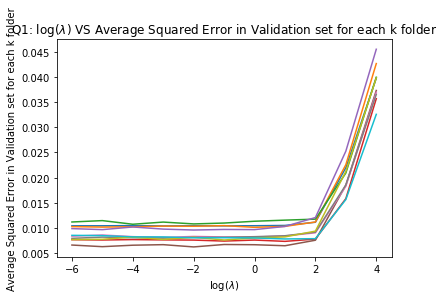
\includegraphics[totalheight=8cm]{q_1.png}
    \caption{Q1: log$(\lambda)$ VS Average Squared Error in valdation set for each k folder}
    \label{fig:verticalcell}
\end{figure}
% \item \emph{( points)} A plot of $\log(\lambda)$ against the squared error in the test data. (10 points)
\\log$(\lambda)$ VS Average Squared Error in valdation set for average of K-folder. Please look at fig.2
\begin{figure}
\centering
        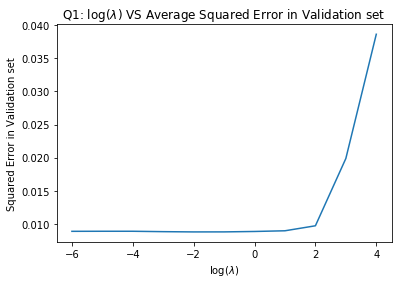
\includegraphics[totalheight=8cm]{q_2.png}
    \caption{Q2: log$(\lambda)$ VS Average Squared Error in valdation set for average of K-folder}
    \label{fig:verticalcell}
\end{figure}
\item 
When $\lambda = 0.01$,\\
The average validation loss is minimum.\\
The best test set proformance: test loss = $4.18$\\
% \item \emph{( points)} A plot of $\lambda$ against the number of small coefficients (you can set a threshold), and a brief commentary on the task of selecting $\lambda$. (15 points)
\item
Please look at fig.3\\ 
The threshold is equal to $10^{-4}$.\\
When $\lambda = 0.01$, the number of small coefficients is not large, so it can keep more features. Therefore $\lambda = 0.01$ is reasonable
\begin{figure}
\centering
        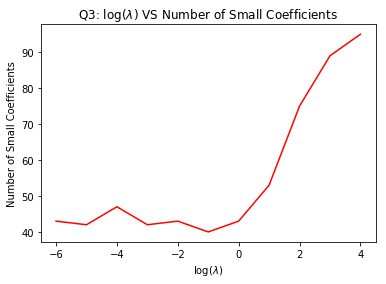
\includegraphics[totalheight=8cm]{q_3.png}
    \caption{Q3: log$(\lambda)$ VS Number of Small Coefficients}
    \label{fig:verticalcell}
\end{figure}
% \item \emph{( points)} For the $\lambda$ that gave the best test set performance, which variable had the largest (most positive) coefficient? What about the most negative? Discuss briefly.  (10 points)
\item 
When $\lambda = 0.01$,\\
The best test set proformance: test loss = $4.18$\\
The largest coefficient: \\
  name: \textbf{PctIlleg}, value: -0.019\\
The smallest coefficient: \\
  name: \textbf{PctKids2Par}, value: -0.01
\end{enumerate}




\end{document}